\chapter{Foundations}
\label{cha:foundations}

This chapter provides descriptions of the concepts used in this thesis.
Section \ref{sec:foundation_decentralized_identities} describes decentralized identities
which are the focus of the research project BestRentalPoC.
Section \ref{sec:foundation_observability} describes observability and monitoring which are
the focus of this thesis.
Section \ref{sec:foundation_devops} and \ref{sec:foundation_cicd} describe the concepts
of DevOps and CI/CD which are used in the results provided by this thesis.

\section{Decentralized Identities}
\label{sec:foundation_decentralized_identities}

Decentralized identities can be broken up into two parts: DIDs (Decentralized Identifiers) and VCs (Verifiable Credentials).
DIDs identify a subject while VCs make claims about the subject. A DID in combination with a set of VCs represents
a decentralized identity.
The W3C (World Wide Web Consortium) provides the standards necessary for the implementation and realization
of decentralized identities.
The standard concerning DIDs is the W3C Recommendation Decentralized Identifiers (DIDs) v1.0 \cite{W3C-DID}
and the standard for VCs is the W3C Working Draft Verifiable Credentials Data Model v2.0 \cite{W3C-VC}.

Identifiers are used to uniquely identify something by a single value.
An everyday example of this is an address that uniquely identifies a place.
Most types of identifiers require a centralized registration authority that issues the identifiers.
The task of the registration authority is to keep track of issued identifiers to ensure their uniqueness
as well as their validity. DID are identifiers that do not require
a centralized registration authority which is often accomplished with cryptography.
In the case of the W3C standards, a DID is a URI that resolves to a DID document.
A DID document contains the information necessary to authenticate the subject of a DID.
Additionally, a DID document contains information about its DID controller which is the entity
that can alter the DID document. The DID controller might also be the subject of the DID.
To resolve a DID, DIDs are entered into a verifiable data registry which records the location
of a DID document corresponding to a DID. Any system that can resolve DIDs to their DID documents
is a verifiable data registry but verifiable data registries are most commonly implemented as
distributed ledgers, peer-to-peer networks, decentralized file systems, databases, and other
forms of trusted decentralized data storage.

A credential is a set of claims made by an issuer regarding one or more subjects.
Each claim is an assertion regarding a subject.
For example, a credential might be a driving license. In this case, the issuer is a driving license authority,
the subject is the holder of the driving license and the claim is that the subject is legally allowed to drive.
VCs are a type of credential with additional properties.
They are tamper-evident, meaning that attempts to modify a VC can be detected.
Additionally, their authorship can be cryptographically verified which means that anybody can verify a VC's issuer
to check the validity of the VC.

Decentralized identities provide improved privacy by minimizing the amount of PII (personally identifiable information)
that needs to be shared. An example of this is a digital driving license, implemented as a decentralized identity,
where a person does not have to share their PII but a third party can still validate
that they possess a valid driving license. Due to their cryptographic nature,
decentralized identities also provide tamper-proof identities along with increased data security.

The following is an example of the usage of decentralized identities.
Alice is a citizen who wants to rent a car. Alice has a DID that uniquely identifies her.
She also has a digital wallet associated with her DID that she can use
to store VCs. Bob is a clerk for a driving license authority.
In order for Alice to be able to rent a car online, she needs a method of proving that she has a valid
driver's license. She goes to Bob and asks him to issue her a Verifiable Credential (VC) for her driving
license, which she could use as proof of her possession of a valid driver's license.
Bob verifies that Alice has a valid driver's license and then issues her the VC using her DID.
The VC is stored in Alice's digital wallet which only she has access to.
When she now goes through the process of renting a car online, the rental company
can ask her to provide a VC to prove that she has a valid driver's license.
Alice can then share her VC from her wallet with the rental company, which can then be
verified by the rental company. The rental company now knows that Alice has a valid driving license.
Alice can now proceed with renting a car online from the rental company.

\section{Observability and Monitoring}
\label{sec:foundation_observability}

In 1960, Kalman \cite{Ka60} defined a system to be observable if its exact state at any time can be completely determined
by its outputs. Based on this definition, observability
for modern cloud systems is the practice of capturing outputs from a software system to
infer knowledge about its state. According to Usman et al. \cite{UF+22}, observability consists of capturing
three main types of data from a system: logs, metrics and traces, these are often called the
three pillars of observability.

Logs are streams of textual information emitted by an application. They can contain information about important
events, like an incoming request, or provide details about the occurrence of exceptions.
Traces are a way of tracking the path of requests through a system. A trace contains detailed information
about all the services that were called during the processing of a request and can be thought of
as a stack trace for microservices.
Metrics are numerical data captured from an application from which the state of the application
can be gauged. An example of a metric is the memory usage of an application.
Because of the scope of this work, from now on, only metrics will be considered for observability.
According to Beyer et al. \cite{BJ+16}, monitoring can be used to capture the four golden signals of
a network-based application. These four signals are Latency, Traffic, Errors, and Saturation.
Latency measures the time that it takes the application to service a request starting from its arrival.
Traffic measures the number of incoming requests per second. Errors are the percentage-based rate at which
incoming requests result in an error. Saturation is a measurement of how much capacity of a constrained
resource like memory is being used and how much is still free.

\begin{figure}[tb]
	\centering
	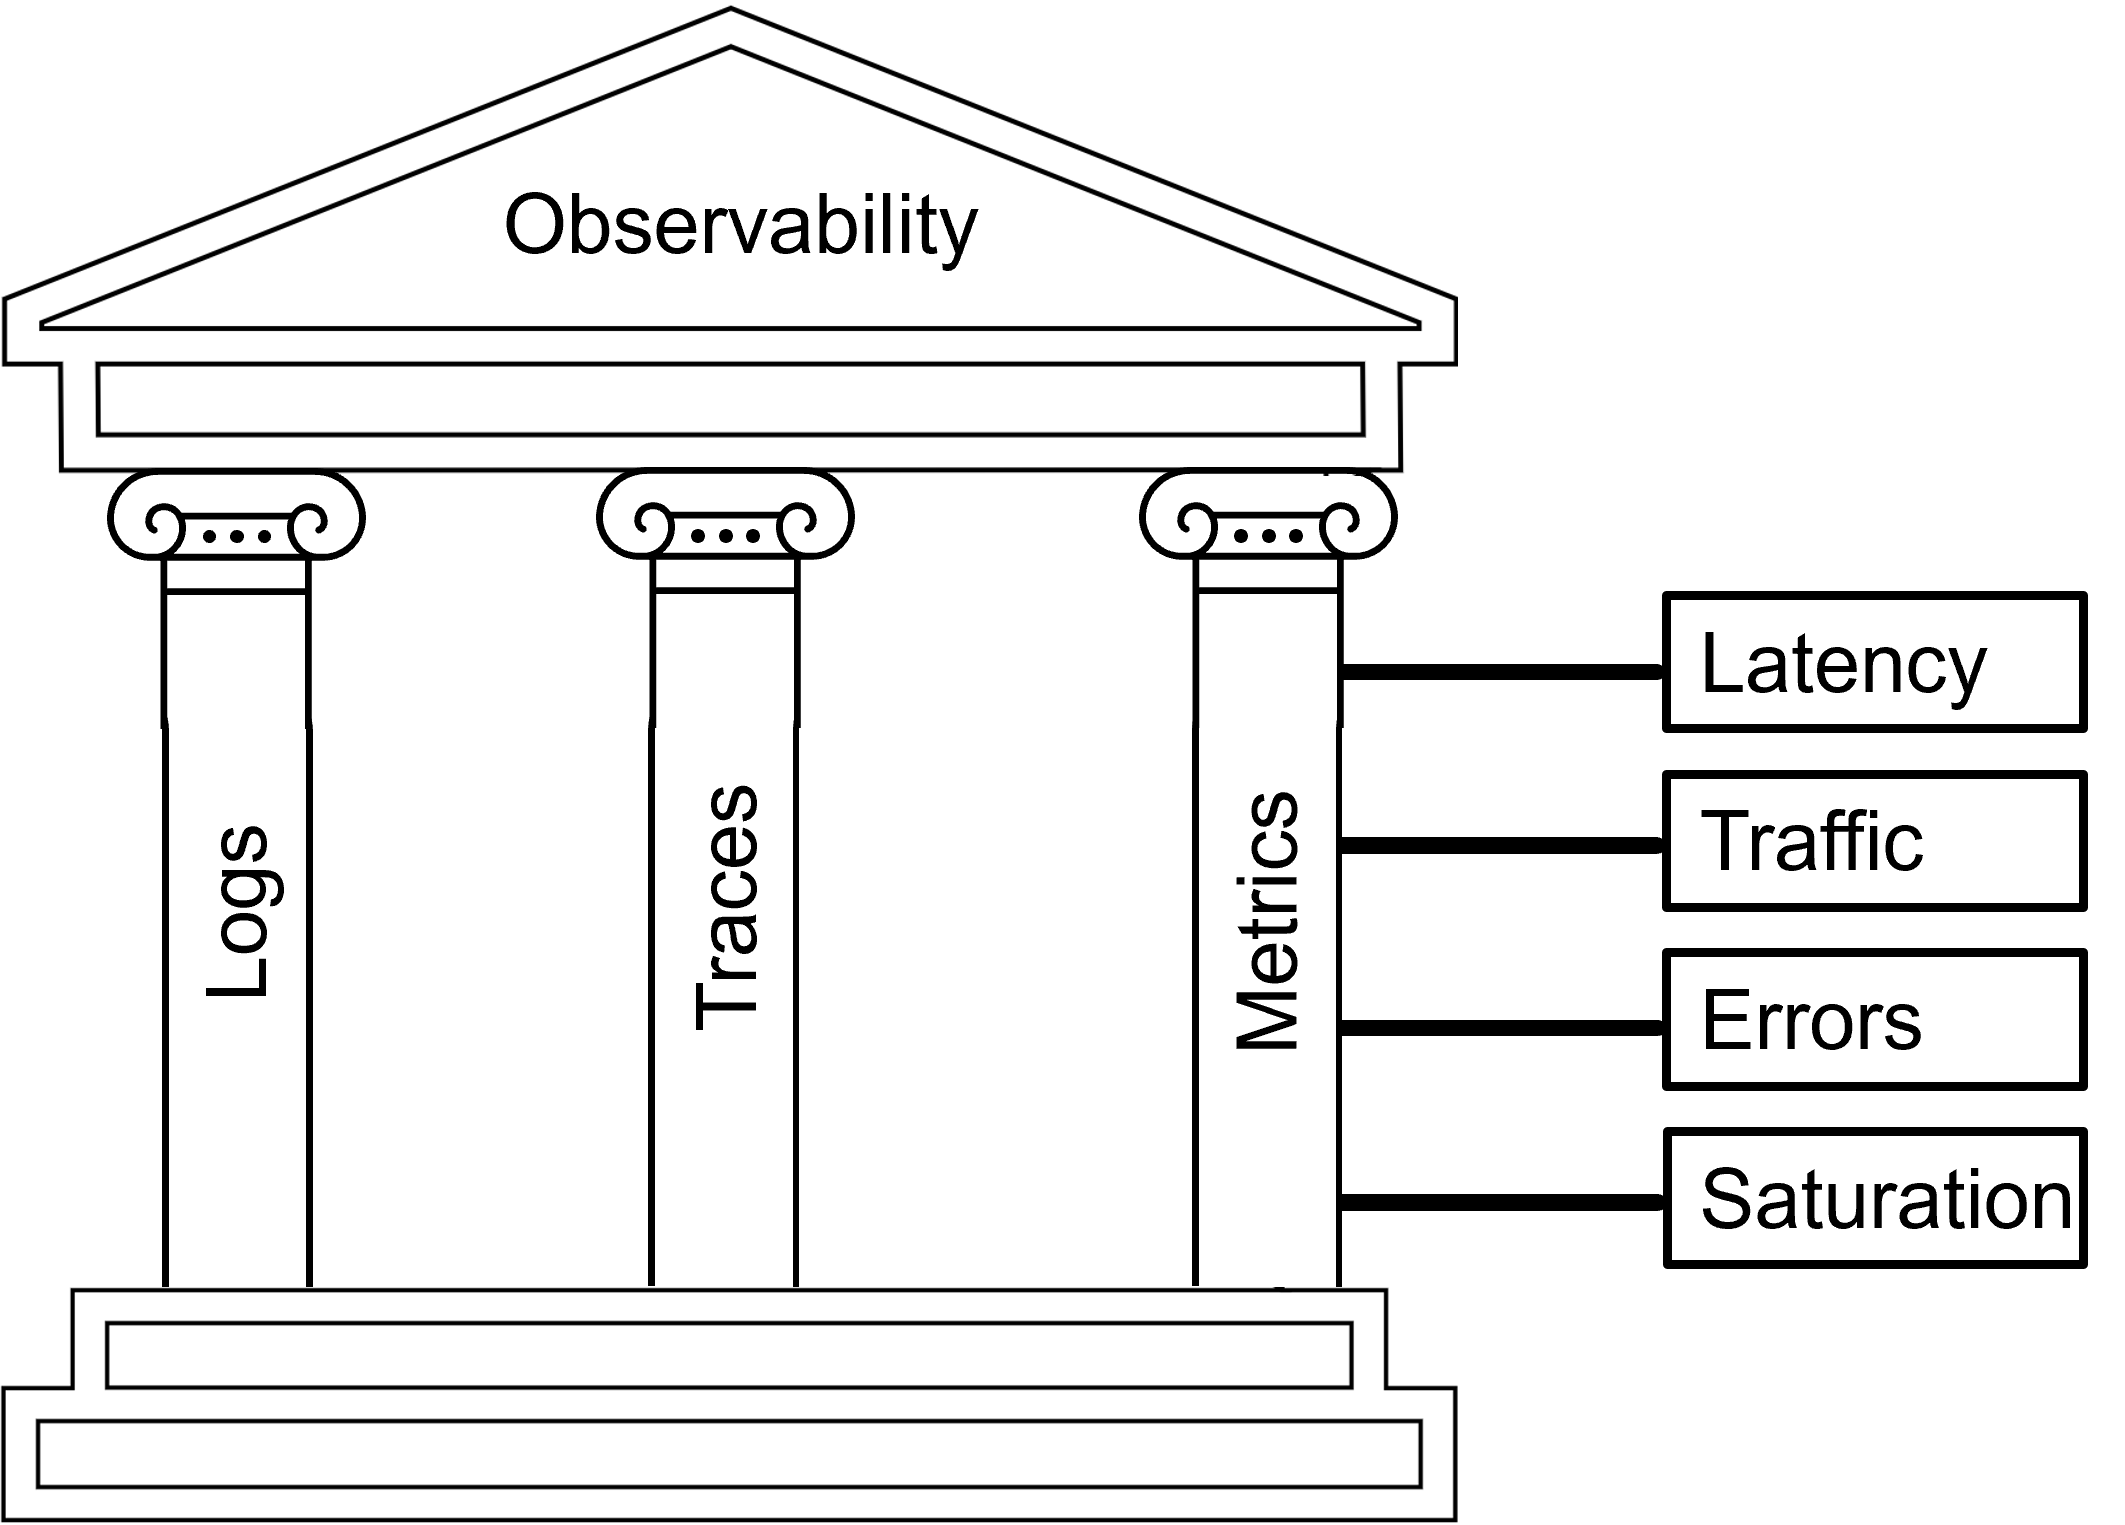
\includegraphics[width=0.7\textwidth]{figures/observability_and_golden_signals.png}
	\caption{Observability and the Four Golden Signals}
	\label{fig:observability_and_golden_signals}
\end{figure}

Beyer et al. \cite{BJ+16} divide monitoring into two categories: white-box and black-box monitoring.
A monitoring approach belongs to the white-box category when it is only based on information that is
internal to the system being monitored. Contrary, a monitoring approach belongs to the black-box category
when it is only based on the externally visible behavior of the system.
Internal resources describe resources that allow direct access to their internals.
An example of an internal resource is a self-hosted microservice.
External resources describe resources that do not allow direct access to their internals.
An example of an external resource is a Software-as-a-Service (SaaS) product which is used in a context that should be monitored.
External resources can, because of their nature, only be monitored using the Black-box approach.
Internal resources however can be monitored with both the White-box and Black-box approach.

Aceto et al. \cite{AB+12} define eight motivations for monitoring cloud applications:
Capacity and Resource Planning, Capacity and Resource Management, Data Center Management,
SLA Management, Billing, Troubleshooting, Performance Management, and Security Management.
Capacity and Resource Planning concerns the resources needed to run an application.
Capacity and Resource Management is Capacity and Resource Planning during the operations
of an application. Metrics allow operators to know if more resources are needed.
Data Center Management is mainly concerned with the efficient usage of resources.
One key measurement of the efficiency of a data center is its energy efficiency.
SLA Management refers to the monitoring of parameters, which are defined in Service Level Agreements (SLA).
These parameters must be within set bounds for an SLA to be considered fulfilled.
Billing refers to the monitoring of parameters that influence the cost of running an application.
When an application is hosted on a cloud provider's Infrastructure-as-a-Service (IaaS) system,
one of those parameters might be the number of compute instances that an application uses.
While Troubleshooting usually refers to the tracing of requests and failures to provide a dataset for analyzing and fixing issues in an application,
Monitoring can also be used to aid in troubleshooting by recording the number of failed requests and their context.
Performance Management captures the performance of an application with metrics like
latency to gauge if the application performs as expected or needs adjustments.
Security Management tracks security-related issues with metrics to allow developers to understand
the source of security issues to mitigate them.

\section{DevOps}
\label{sec:foundation_devops}

DevOps (Development and Operations) is a philosophy for developing software.
It provides practices and principles which aim to enhance the collaboration
between software development and its operation which in turn should increase
the overall efficiency of the software development process.

DevOps is based on the agile approach to project management.
Agile project management turns linear processes into iterative ones.
An example of a linear process is the waterfall model for software development in which
the different phases of development happen one after another.
In an iterative process, the work is split into multiple packages
which are completed in order. For each process, there is a complete linear work process.
This results in multiple processes which are iteratively completed.
The principles of agile project management can also be applied to software development
to get an iterative development process.
DevOps takes this iterative approach and expands on it through faster cycle times of
building and shipping a new version of an application.
To achieve this, DevOps focuses on increasing the efficiency of cross-functional
collaborations between developers and operators with four core principles \cite{GIT-DEV}.
The first principle is automation. According to DevOps, everything that is needed
to deliver software to a customer should be automated. On the development side, this includes
testing and building. On the operations side, this includes provisioning infrastructure
and deploying software as well as monitoring it. DevOps commonly employs CI/CD to achieve this.
The second principle is collaboration. Commonly, teams, which participate in the
development process of a software project, are split into two categories:
Development teams, which only focus on the development of the software,
and operation teams, which focus on its deployment and operation.
To increase the cooperation between participants, DevOps reorders teams to have both
developers and operators. In this configuration, each team is responsible for the whole process
of its contribution from development to operations.
The third principle is the focus on continuous improvements and minimization of waste
in the form of time and money. DevOps employs monitoring and the measurement of metrics
for this task.
The fourth principle is the focus on the customer's needs. One advantage of an iterative process
compared to a linear one is that changes requested by a customer can be adopted faster.
In a linear process, the whole process would have to be started from the beginning to adopt changes.
An iterative process can adopt changes in its next iteration step which, compared
to the overall length of the complete process, takes less time.
Lwakatare et al. \cite{LK+16} sort these principles into the five dimensions
Collaboration, Automation, Culture, Monitoring, and Measurement where the third DevOps
principle spans the dimensions of Monitoring and Measurement. The dimension of
Culture adds additional focus on the principle of collaboration by stating that
joint responsibility is necessary for the success of the collaboration between
developers and operators. Joint responsibility ensures that all persons involved
have the common interest of maintaining the quality of the software that they are developing.
The combination of these principles and dimensions into DevOps promises faster
development times for software while simultaneously improving its quality thus
resulting in an overall efficiency gain for the development process.
% TODO: This needs a citation

\section{CI/CD}
\label{sec:foundation_cicd}

CI/CD (Continuous Integration/Continuous Deployment) is a part of DevOps
and combines continuous integration with continuous delivery and deployment to
achieve the DevOps principle of automation. Generally speaking,
CI/CD tries to reduce the amount of human involvement needed after a developer has written
source code. This means automating the building and testing of that code which is referred
to as continuous integration as well as the deployment and infrastructure provisioning
for the deployment which is continuous deployment. Sometimes CD also refers to
continuous delivery instead of deployment. In this case, CI/CD stops before the deployment
of the software and ends with end-to-end tests of the system after integrating changes.

CI/CD has eight fundamental elements \cite{GIT-CICD}.
The first two elements are a single source repository and frequent check-ins to the main branch.
This practice reduces the number of duplicated artifacts, makes configuration easier and
works to reduce the number of merge conflicts.
Elements number three and four are automated and self-testing builds.
Automated builds reduce the amount of human involvement necessary while automated testing ensures
the software's quality. Element five supports automated testing with stable testing environments
that are clones of the live production environment.
Element six adds to the second element with frequent iterations which reduces the size of changes
from each iteration making it easier to identify problems and roll them back.
Element seven is maximum visibility. Every developer should be able to access all artifacts from
the development process to make the identification of concerns easier and more likely.
The last element is predictable deployments at any time. This ensures that should a problem arise
in a production environment, it can easily be rolled back with confidence.
Overall this approach promises faster times until the customer receives value, less context switching
from working with multiple different sources and fast recovery in case of problems.